\documentclass{article}[18pt]
\usepackage{/home/sam/Documents/School_Notes/format}
\lhead{A Level Physics - Fields}

\begin{document}
\begin{center}
\underline{\huge Electric Fields Notes}
\end{center}

\begin{obeylines}
\section{Static Electricity}
\textbf{Like charges repel; unlike charges attract}
Electrical conductors have many free electrons, these can move in the material and are not attached to any atom. To charge a metal, it must be isolated from the earth to stop the charge being neutralised by electrons from the earth. It can then be charged by direct contact with a charged object. If an isolated conductor is charged then earthed, the electrons will transfer to neutralise it.  
Electrically insulating materials do not contain free electrons, all electrons are attached to atoms. Some insulators can be charged easily because their surface atoms easily gain or lose electrons.

A \textbf{gold leaf electroscope} is used to detect charge. If it is in contact with charge the gold leaf and the metal stem have the same charge and so repel.
\section{Shuttling ball experiment}
A ball swinging between one positively charged plate and one negatively charged plate will lose electrons at the positive plate and so be repelled towards the negative plate where it will pick up electrons and gets repelled away, and so the process repeats.
\section{Field lines and patterns}
Electric fields surround each charged object, if a small charged object is placed near a larger same charged object the path the small charge will follow is called a \textbf{line of force} or \textbf{field line}. The direction of an electric field is the direction the charge moves.
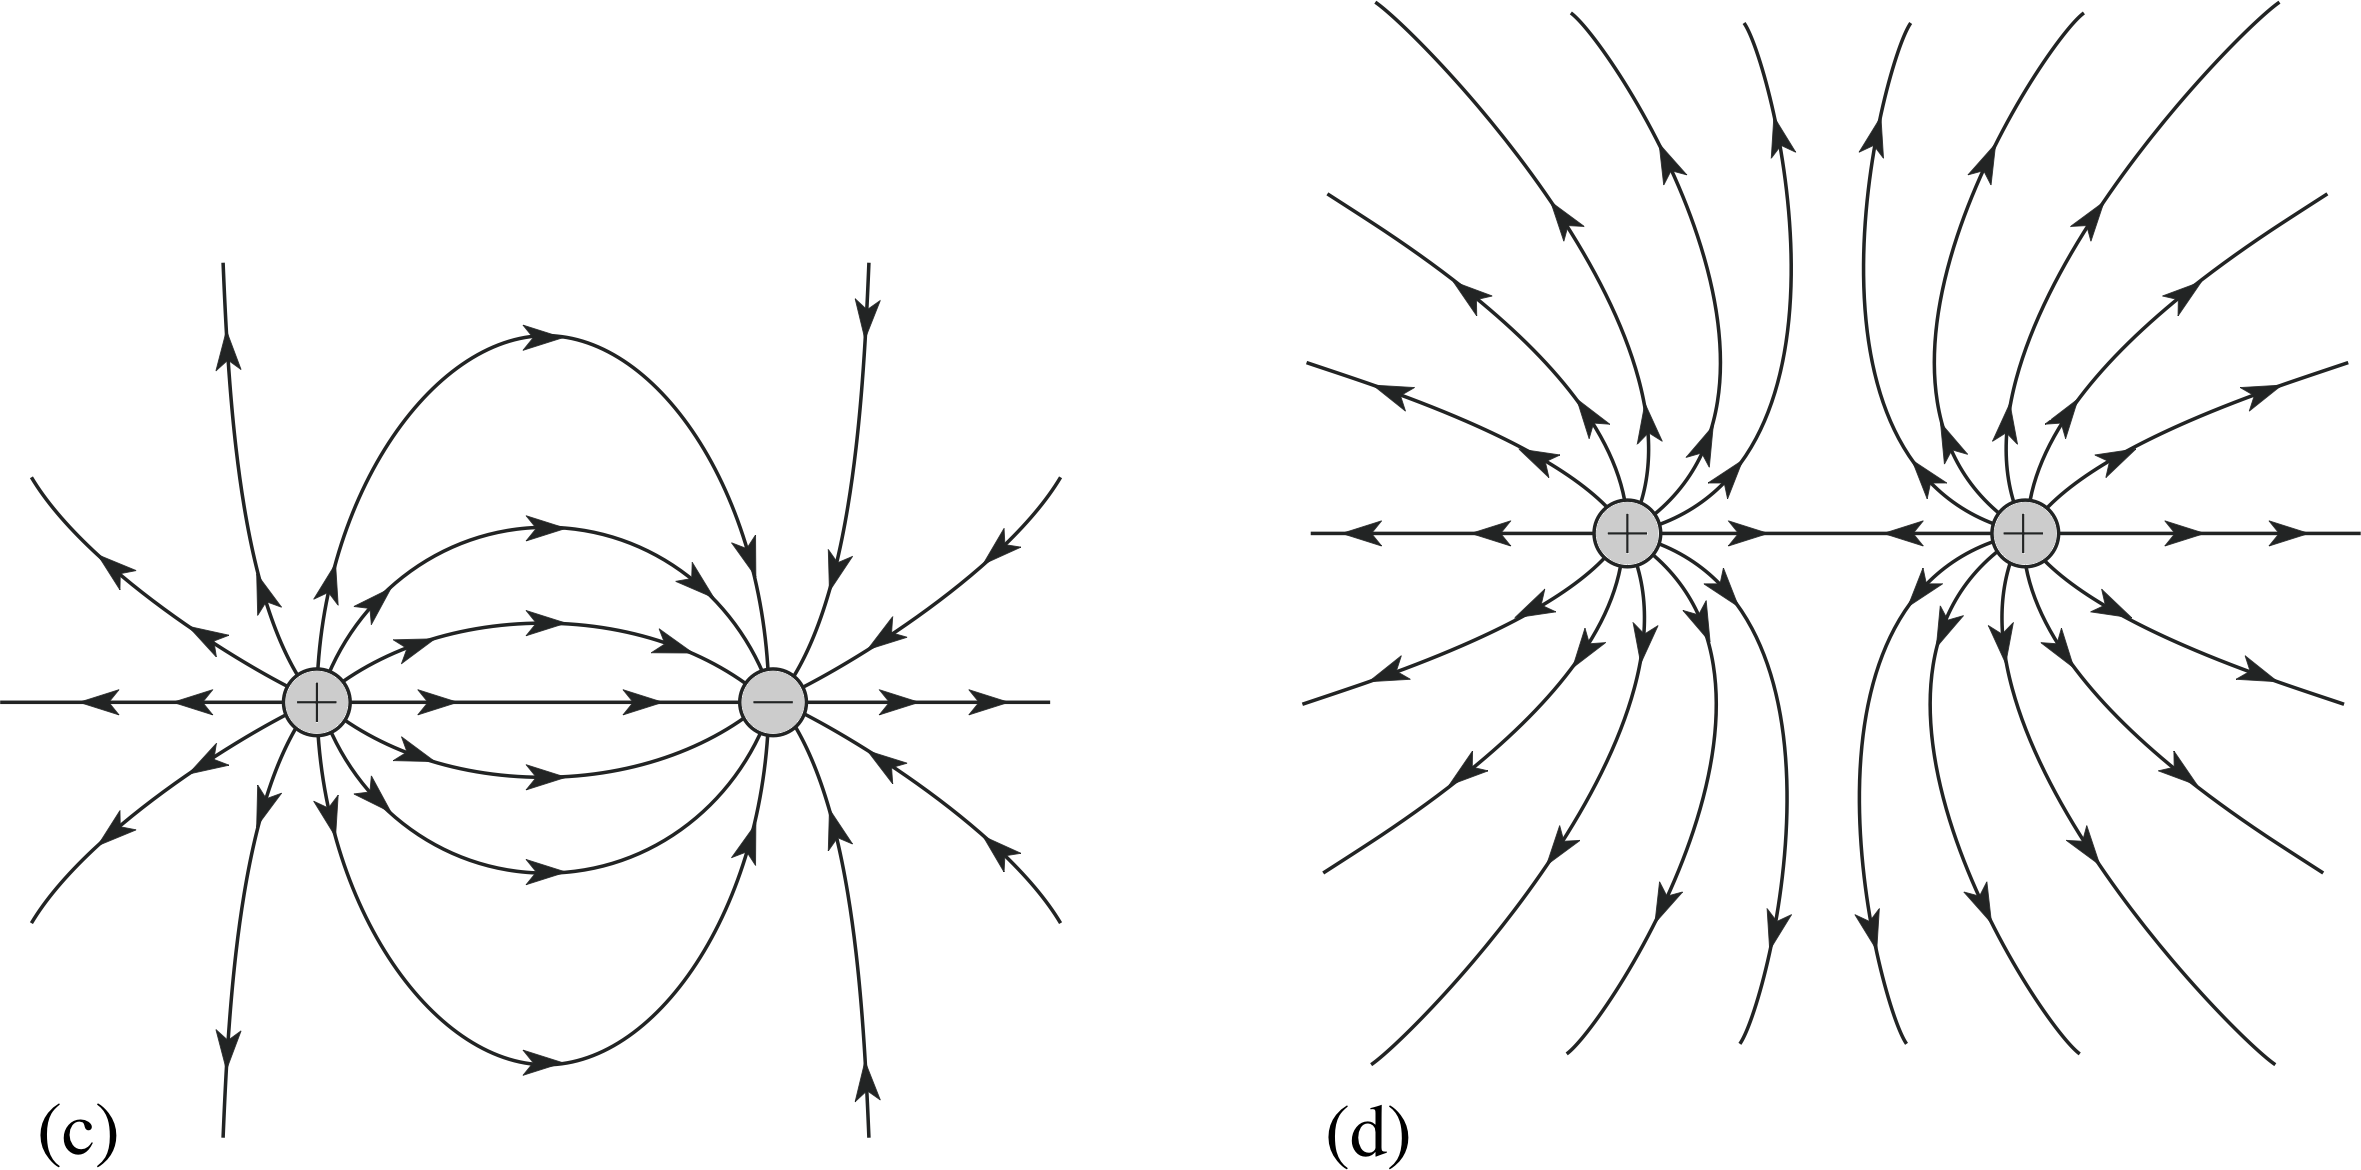
\includegraphics[width=5in]{field_lines.png}
\section{Electric field strength}
The field strength of a uniform field is constant at all points.
The electric field strength, E, at a point in the field is defined as the force per unit charge on a positive test charge placed at that point.
The unit of electric field strength is Newton per coulomb $NC^{-1}$
If a positive charge of \textbf{Q} us acted on by a force \textbf{F} the electric field strength at that point is 
$E=\dfrac{F}{Q}$
\section{The electric field between two parallel plates}
Field lines between two parallel plates are:
\begin{itemize}
\item Parallel to each other
\item At right angles to the plates
\item From the positive plate to the negative plate
\item Uniform
\end{itemize}
$E=\dfrac{V}{d}$
V=Potential difference between plates
d= Separation between plates
Proof:
$F=QE$
$Work done= Force \times Distance$
$d=QEd$
$ $
$V=\dfrac{W}{Q}=\dfrac{QEd}{Q}=Ed$
$ $
$E=\dfrac{V}{d}$
\section{Field Factors}
The greater the charge on a body, the stronger the electric field is. The more concentrated the charge is on the surface, the greater the strength of the electric field is above the surface.
For a charge,\textbf{Q}, on a plate of surface area,\textbf{A}, the electric field is proportional to $\dfrac{Q}{A}$ 
Including a constant of proportionality the equation gives $\dfrac{Q}{A}=\epsilon_0E$
The unit of $\epsilon_0$ is $Fm^{-1}$ and is called the \textbf{Permittivity of free space} as it represents the charge per unit area on a surface in a vacuum that produces an electric field strength of one volt per one metre between the plates.
\section{The Van de Graff generator}
A Van de Graff generator works by rubbing a rubber belt against a pad up to a metal dome. This increased the PD between the dome and the earth until sparks start. 
The electric potential at a certain position in any electric field is defined as the work done per unit charge on a positive test charge when it is moved from infinity to that position. 

$E_P=QV$ or $V=\dfrac{E_P}{Q}$

\section{Potential gradients}
Equipotentials are surfaces of constant potential. A test charge moving along an equipotential has constant potential energy. The \textbf{potential gradient} at any position in an electric field is the change in potential per unit change of distance in a given direction.
If the field is \textbf{non-uniform} the potential gradient varies according to position and direction. The closer the equipotentials are, the greater the potential gradient at right angles to the equipotentials. 
If the field is \textbf{uniform} the equipotentials between the plates are equally spaced lines parallel to the plates.
In a uniform field the potential gradient is 
\begin{itemize}
\item Constant
\item Potential increases in the opposite direction to the electric field
\item Equal to $\dfrac{V}{d}$
\end{itemize}
\textbf{The electric field strength is equal to the negative of the potential gradient}
The potential gradient at any position in an electric field is $\dfrac{\Delta V}{\Delta x}$ where $\Delta V$ is the potential difference between two points and $\Delta X$ is the distance between the points.
$E=-\dfrac{\Delta V}{\Delta X}$
\newpage
\section{Coulomb's law}
$F=\dfrac{KQ_1Q_2}{r^2}$
F=Force between two point charges
K=$\dfrac{1}{4\pi\epsilon_0}$
$Q_1$=Point charge 1
$Q_2$=Point charge 2
r=Distance between the two point charges

$F=\dfrac{1}{4\pi\epsilon_0}\dfrac{Q_1Q_2}{r^2}$
\section{Charged particles in electric fields}
\subsection{Force}
Force is the same throughout the journey.
Calculated by
\begin{itemize}
\item $f=EQ$
\item $E=\dfrac{V}{d}$
\end{itemize}
\subsection{Velocity}
Horizontal velocity is constant
Vertical velocity increases as the particle passes through the field
\section{Point charges}
A point charge is a charge where the distances considered are much larger than the object, meaning the charge can be thought of as being in one place.
The electric field strength at a distance r from Q is:
$E=\dfrac{Q}{4\pi\epsilon_0r^2}$
\textit{Note that Q is negative}
\subsection{Example Field strength question}
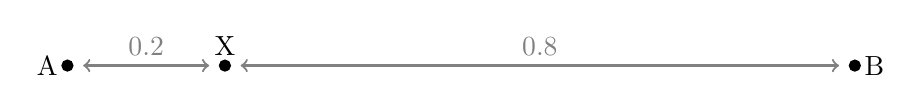
\begin{tikzpicture}
\draw[gray, thick,<->] (-1.8,0) -- (-0.2,0) node[above,midway] {0.2};
\draw[gray, thick,<->] (0.2,0) -- (7.8,0) node[above, midway] {0.8};
\filldraw[black] (0,0) circle (2pt) node[anchor=south] {X};
\filldraw[black] (-2,0) circle (2pt) node[anchor=east] {A};
\filldraw[black] (8,0) circle (2pt) node[anchor=west] {B};
\end{tikzpicture}
\textit{Find the field strength at the point X, the charge at A and B is $4\mu C$}\\
E at X due to A
$$\frac{1}{4\pi\epsilon_0}\times\frac{4\times10^{-6}}{0.2^2}=8.99\times10^5NC^{-1} \quad \textrm{Left to right}$$ 
E at X Due to B
$$\frac{1}{4\pi\epsilon_0}\times\frac{4\times10^{-6}}{0.8^2}=5.62\times10^4NC^{-1} \quad \textrm{Right to left}$$ 
Total E at X
$$8.99\times10^5-5.62\times10^4=8.43\times10^5NC^{-1}\quad \textrm{Left to right}$$
\newpage
\subsection{Example Electric Potential}
\textbf{For electric potential, ignore which side of the point the charge is on}
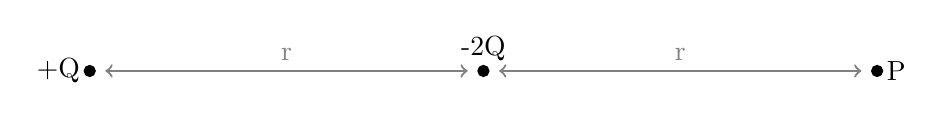
\begin{tikzpicture}
\draw[gray, thick,<->] (-4.8,0) -- (-0.2,0) node[above,midway] {r};
\draw[gray, thick,<->] (0.2,0) -- (4.8,0) node[above, midway] {r};
\filldraw[black] (0,0) circle (2pt) node[anchor=south] {-2Q};
\filldraw[black] (-5,0) circle (2pt) node[anchor=east] {+Q};
\filldraw[black] (5,0) circle (2pt) node[anchor=west] {P};
\end{tikzpicture}
\textit{Find the electric potential at P}\\
Electric potential due to +Q charge
$$V=\frac{1}{4\pi\epsilon_0}\times\frac{Q}{2r}$$
Electric potential due to -2Q charge
$$V=\frac{1}{4\pi\epsilon_0}\times\frac{-2Q}{r}$$
Add two equations
$$V=\frac{1}{4\pi\epsilon_0}\Bigg(\frac{Q}{2r}-\frac{2Q}{r}\Bigg)$$
Simplify
$$V=\frac{1}{4\pi\epsilon_0}\times\frac{-3Q}{2r}$$




\section{Electric field strength as a vector}
In general, the electric field strength is the vector sum of the individual electric field strengths
\subsection{Forces in the same direction}
$F=F_1+F_2=qE_1+qE_2$
Therefore $E=\dfrac{F}{q}=\dfrac{qE_1+qE_2}{q}=E_1+E_2$
\subsection{Forces in opposite directions}
$F=F_1-F_2=qE_1-qE_2$
Therefore $E=\dfrac{F}{q}=\dfrac{qE_1-qE_2}{q}=E_1-E_2$
\subsection{Forces at right angles to each other}
$F^2={F_1}^2+{F_2}^2$
$E=\dfrac{F}{q}$
$E^2={E_1}^2+{E_2}^2$
\section{More about radial fields}
The electric field lines surrounding a point charge are radial.
Coulomb's law and Newton's law are similar as they have inverse square relationships.
The equation for electric potential near a point charge and gravitational potential near a point mass are also very similar.
\section{The relationship between electric field strength and electric potential}
Electric field strength = -gradient of a potential vs distance graph. 
Change in potential = Area under an electric field vs distance graph.
\end{obeylines}


\section{Comparing electric fields and gravitational fields}
\begin{tabular}{ |p{5.5cm}|p{5.5cm}|p{5.5cm}|  }
\hline
&Gravitational Fields&Electrostatic fields\\
 \hline
 \multicolumn{3}{|c|}{Similarities} \\
 \hline
 Line of force&Path of a free test mass in the field & Path of a free test charge in the field\\
 \hline
 Inverse square law of gravitation & Newton's law of gravitation & Coulomb's law of force\\
 \hline
 Field strength & $g=\dfrac{F}{m}$ & $E=\dfrac{F}{q}$\\
 \hline
 Unit of field strength & $Nkg^{-1}$ or $ms^{-2}$ & $NC^{-1}$ or $Vm^{-1}$\\
 \hline
 Uniform fields & G is the same everywhere and field lines are parallel and equally spaced & E is the same everywhere and field lines are parallel and equally spaced \\
 \hline
 Unit of potential & $Jkg^{-1}$ & $JC^{-1}$ \\
 \hline
 Potential energy of two point mass or charges & $E_P=\dfrac{-Gm_1m_2}{r}$ & $E_P=\dfrac{Q_1Q_2}{4\pi\epsilon_0r}$\\
 \hline
 \multicolumn{3}{|c|}{Differences} \\
 \hline
 Action at a difference & Between any two masses & Between two charged objects \\
 \hline
 Force & Attracts only & Unlike charges attract; like charges repel \\
 \hline
 Constant of proportionality in force law & G & $\dfrac{1}{4\pi\epsilon_0}$ \\
 \hline
 
 
\end{tabular}












\end{document}